%%%%%%%%%%%%%%%%%%%%%%%%%%%%%%%%%%%%%%%%%%%%%%%%%%%%%%%%%%%%%%%%%%%%%%
% Lớp 11 | Hàm số lượng giác và phương trình lượng giác | Góc lượng giác
% Dạng 1D1?1-4: Độ dài của một cung tròn
% Số câu: 55  (sinh tự động bởi tach_cau.py; từ nay thầy sửa trực tiếp file này)
%%%%%%%%%%%%%%%%%%%%%%%%%%%%%%%%%%%%%%%%%%%%%%%%%%%%%%%%%%%%%%%%%%%%%%

%%%%%%%%%%%%%%%% TRẮC NGHIỆM 4 PHƯƠNG ÁN %%%%%%%%%%%%%%%%

% nguồn: Ok_Toan11_TracNghiem_Lan2
\begin{ex}%[1D1N1-4]%[ma:106748dc]
	Một  đường tròn có bán kính $10$, độ dài cung tròn có góc ở tâm bằng $40^\circ$ gần bằng nhất với giá trị nào sau đây?
	 \choice
		{\True $7$} 
		{$9$} 
		 {$11$}
		 {$13$}
	 \loigiai{
		Ta có  $l=\dfrac{R\alpha\pi}{180^\circ}=\dfrac{40^\circ\cdot10\cdot\pi}{180^\circ}=\dfrac{20\pi}{9} \approx 7$.
	} 
\end{ex}

% nguồn: Ok_Toan11_TracNghiem_Lan2
\begin{ex}%[1D1N1-4]%[ma:b75081a5]
	Trên đường tròn đường kính $8$ cm, tính độ  dài cung tròn có số đo bằng $1{,}5\,\mathrm{rad}$.
	 \choice
		{$12$  cm}
		{$4$ cm} 
		{\True $6$  cm}
		{$15$  cm}
	 \loigiai{
		Tính được $\ell=\alpha  \cdot R=1{,}5\cdot \dfrac{8}{2}=6$ cm.
	} 
\end{ex}

% nguồn: Ok_Toan11_TracNghiem_Lan2
\begin{ex}%[1D1N1-4]%[ma:0612500f]
	Một đường tròn có bán kính $R=\dfrac{10}{\pi}$, độ dài cung tròn $\dfrac{\pi}{2}$ là 
	\choice 
		{\True $5$} 
		{$5\pi$} 
		{$\dfrac{5}{\pi}$} 
		{$\dfrac{\pi}{5}$} 
	\loigiai{ 
		 $$
		\ell=\alpha \cdot R=\dfrac{10}{\pi}  \cdot \dfrac{\pi}{2}=5.
		 $$
	 }
\end{ex}

% nguồn: Ok_Toan11_TracNghiem_Lan2
\begin{ex}%[1D1N1-4]%[ma:b59806f8]
	Cho $\alpha$ thuộc góc phần tư thứ nhất  của đường tròn lượng giác. Hãy chọn kết quả đúng trong các kết quả sau đây.
	\choice 
		 {$\sin \alpha >0$}
		{$\cos \alpha  <0$}
		{$\tan \alpha  <0$}
		{$\cot \alpha <0$} 
	\loigiai{ 
	$\alpha $ thuộc góc phần tư thứ nhất  $\Rightarrow \heva{&\sin \alpha >0 \\ &\cos \alpha >0 \\ &\tan \alpha >0 \\&\cot \alpha >0.}$}
\end{ex}

% nguồn: Ok_Toan11_TracNghiem_Lan2
\begin{ex}%[1D1N1-4]%[ma:c7e4d922]
	Cho $2\pi <\alpha <\dfrac{5\pi}{2}$.  Chọn mệnh đề đúng.
	\choice 
		 {\True $\tan \alpha >0$}
		{$\cot  \alpha <0$}
		{$\sin \alpha  <0$}
		 {$\cos \alpha <0$}
	\loigiai{ 
	Ta có  $2\pi <\alpha <\dfrac{5\pi}{2}$ nên $\tan \alpha >0$.}
\end{ex}

% nguồn: Ok_Toan11_TracNghiem_Lan2
\begin{ex}%[1D1N1-4]%[ma:9aafea7b]
	Cho $\pi <\alpha  <\dfrac{3\pi}{2}$, tìm phát biểu đúng trong các phát biểu sau.
	\choice 
		 {$\sin x>0$}
		{$\cos  x>0$}
		{\True $\tan  x>0$}
		{$\cot x<0$} 
	 \loigiai{
	Ta có $\pi <\alpha <\dfrac{3\pi}{2}\Rightarrow \heva{&\sin x<0 \\&\cos x<0 \\&\tan x>0  \\&\cot x>0 .}$}
\end{ex}

% nguồn: Ok_Toan11_TracNghiem_Lan2
\begin{ex}%[1D1N1-4]%[ma:f6af0fd7]
	Cho góc $\alpha $ thỏa $-\dfrac{3\pi}{2}<\alpha <-\pi  $. Tìm mệnh đề đúng trong các mệnh đề sau.
	 \choice
		{$\cos \alpha  >0$}
		{$\cot  \alpha >0$}
		{\True $\sin \alpha >0$} 
		{$\tan \alpha  >0$}
	\loigiai{ 
	\immini 
		{Vì $-\dfrac{3\pi}{2}<\alpha <-\pi $ nên điểm $M$ biểu  diễn cung $AM$ có số $\alpha $ thuộc góc phần tư số II.\\
		Do đó $\sin \alpha >0$,  $\cos \alpha <0$, $\tan \alpha <0$, $\cot \alpha <0$.}
		{ 
		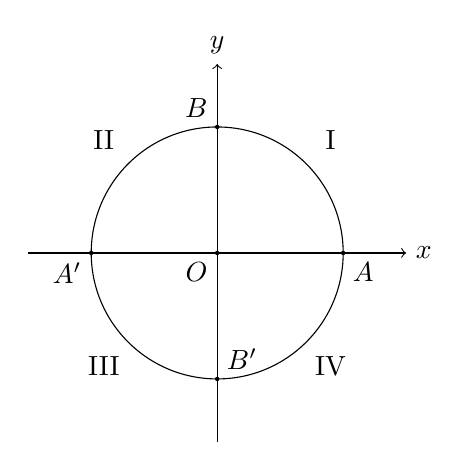
\begin{tikzpicture}[scale=0.8]
				\draw[->] (-3,0)  -- (3,0) node[right] {$x$};
				\draw[->] (0,-3)  -- (0,3) node[above] {$y$};
				\draw  (0,0) circle (2);
				 \coordinate (A) at (2,0);
				\coordinate (B) at  (0,2);
				 \coordinate (A') at (-2,0);
				\coordinate (B') at (0,-2); 
				\fill (A) circle (1pt) node[below right] {$A$}; 
				\fill (B) circle (1pt) node[above  left] {$B$};
				\fill (A') circle (1pt) node[below left] {$A'$}; 
				\fill (B') circle (1pt)  node[above right] {$B'$};
				 \node at (1.8,1.8) {I};
				\node  at (-1.8,1.8) {II};
				 \node at (-1.8,-1.8) {III};
				 \node at (1.8,-1.8) {IV};
				\fill (0,0) circle (1pt) node[below left]  {$O$};
			\end{tikzpicture}
		 }
	} 
\end{ex}

% nguồn: Ok_Toan11_TracNghiem_Lan2
\begin{ex}%[1D1N1-4]%[ma:aee01f4e]
	Một đường tròn có bán kính $15$ cm. Độ dài cung tròn có  góc ở tâm bằng $30^\circ$ là
	 \choice
		{\True $\dfrac{5\pi}{2}$ cm} 
		{$\dfrac{5\pi}{3}$  cm}
		 {$\dfrac{2\pi}{5}$ cm}
		{$\dfrac{\pi}{3}$  cm}
	 \loigiai{
		Ta có $l=\dfrac{R\alpha\pi}{180^\circ}=\dfrac{15\cdot 30^\circ\cdot\pi}{180^\circ}=\dfrac{5\pi}{2}$  (cm).
	} 
\end{ex}

% nguồn: Ok_Toan11_TracNghiem_Lan2
\begin{ex}%[1D1N1-4]%[ma:03f319ac]
	Cho góc $\alpha $ thoả mãn $90^\circ <\alpha <180^\circ $.  Trong các khẳng định sau, khẳng định nào đúng?
	\choice 
		{$\sin \alpha <0$} 
		{$\cos\alpha \ge  0$}
		{\True $\tan \alpha <0$} 
		{$\cot\alpha  >0$}
	 \loigiai{
	 Khẳng định đúng là $\tan \alpha <0$.}
\end{ex}

% nguồn: Ok_Toan11_TracNghiem_Lan2
\begin{ex}%[1D1N1-4]%[ma:9578d408]
	Một đường tròn có bán kính $R=\dfrac{10}{\pi}$, độ dài cung tròn có  số đo $\dfrac{\pi}{2}\,\mathrm{rad}$ là
	\choice 
		{\True $5$} 
		 {$5\pi$}
		 {$\dfrac{5}{\pi}$}
		 {$\dfrac{\pi}{5}$}
	\loigiai{ 
		Ta có $l=R\alpha=\dfrac{10}{\pi}\cdot\dfrac{\pi}{2}=5$. 
	 }
\end{ex}

% nguồn: Ok_Toan11_TracNghiem_Lan2
\begin{ex}%[1D1N1-4]%[ma:9a1316f8]
	Cung tròn bán kính bằng $8{,}43$ cm. Độ dài cung có số đo $3{,}85$ rad là 
	\choice 
		 {\True $32{,}46$ cm}
		{$32{,}45$ cm} 
		{$32{,}47$  cm}
		{$32{,}5$ cm} 
	 \loigiai{
		Ta có $l=R\alpha=3{,}85\cdot8{,}43\approx  32{,}46$ (cm).
	 }
\end{ex}

% nguồn: Ok_Toan11_TracNghiem_Lan2
\begin{ex}%[1D1N1-4]%[ma:dc43b889]
	Một đường tròn có bán kính $10$, độ dài cung tròn $40^{\circ}$ trên đường  tròn gần bằng
	\choice 
		 {\True $7$}
		{$9$} 
		 {$11$}
		 {$13$}
	\loigiai{ 
		 $$
		\ell=\dfrac{\pi a \cdot R}{180}=\dfrac{\pi \cdot 40 \cdot 10}{180}=\dfrac{20 \pi}{9} \approx 7. 
		 $$
	 }
\end{ex}

% nguồn: Ok_Toan11_TracNghiem_Lan2
\begin{ex}%[1D1N1-4]%[ma:2c4751b3]
	Cho $\dfrac{\pi}{2}<\alpha <\pi$. Kết quả đúng là 
	 \choice
		 {$\sin \alpha >0$, $\cos \alpha >0$}
		{$\sin  \alpha <0$, $\cos \alpha <0$}
		{\True  $\sin \alpha >0$, $\cos \alpha <0$}
		{$\sin \alpha <0$, $\cos  \alpha >0$}
	 \loigiai{
	Vì $\dfrac{\pi}{2}<\alpha <\pi$  nên $\sin \alpha >0$; $\cos \alpha <0$.}
\end{ex}

% nguồn: Ok_Toan11_TracNghiem_Lan2
\begin{ex}%[1D1N1-4]%[ma:063a73b9]
	Trên đường tròn  bán kính $7$ cm, lấy cung có số đo $54^{\circ}$. Độ dài $\ell$ của cung tròn bằng
	 \choice
		 {\True $\dfrac{21}{10} \pi\,(\mathrm{cm})$}
		 {$\dfrac{11}{20} \pi\,(\mathrm{cm})$}
		 {$\dfrac{63}{20} \pi\,(\mathrm{cm})$}
		 {$\dfrac{20}{11} \pi\,(\mathrm{cm})$}
	 \loigiai{
		Ta có $\ell=7\cdot\left(\dfrac{54^{\circ}}{180^{\circ}} \cdot  \pi\right)=\dfrac{21}{10} \pi\,(\mathrm{cm})$.
	 }
\end{ex}

% nguồn: Ok_Toan11_TracNghiem_Lan2
\begin{ex}%[1D1N1-4]%[ma:2054b4ca]
	Ở góc phần tư  thứ tư của đường tròn lượng giác. hãy chọn kết quả đúng trong các kết quả sau đây.
	\choice 
		{$\tan  \alpha >0$}
		{$\sin \alpha >0$} 
		 {\True $\cos \alpha >0$}
		{$\cot \alpha >0$} 
	 \loigiai{
		Ở góc phần tư thứ tư thì $\sin \alpha <0$, $\cos \alpha >0$,  $\tan \alpha <0$, $\cot \alpha <0$.
	 }
\end{ex}

% nguồn: Ok_Toan11_TracNghiem_Lan2
\begin{ex}%[1D1N1-4]%[ma:dd9d8aaa]
	Trên đường tròn bán kính $7$ cm, lấy cung có số  đo $54^{\circ}$. Độ dài $l$ của cung tròn bằng
	\choice 
		{\True  $\dfrac{21}{10} \pi$ cm}
		{$\dfrac{11}{20} \pi$  cm}
		{$\dfrac{63}{20} \pi$ cm} 
		{$\dfrac{20}{11} \pi$ cm} 
	 \loigiai{
		Ta có  $l=7\cdot\left(\dfrac{54}{180}\cdot\pi \right)=\dfrac{21}{10} \pi$ (cm).
	} 
\end{ex}

% nguồn: Ok_TracNghiemLop11_Lan1
\begin{ex}%[1D1N1-4]%[ma:de2b3498]
	 Trên đường tròn bán kính $R=6$, cung $\alpha=\dfrac{2\pi}{3}$ có độ dài bằng bao nhiêu?
	\choice 
		{$l=2\pi$} 
		{$l=8\pi$} 
		{\True  $l=4\pi$}
		 {$l=6\pi$}
	\loigiai{ 
		Ta có cung có số đo $\alpha=\dfrac{2\pi}{3}$ rad của đường tròn có bán kính $R$ có độ dài $l=R\alpha$.\\ 
	Do đó cung $\alpha=\dfrac{2\pi}{3}$ và có bán kính $R=6$ có độ dài  là $l=6\cdot\dfrac{2\pi}{3}=4\pi$.}
\end{ex}

% nguồn: Ok_TracNghiemLop11_Lan1
\begin{ex}%[1D1N1-4]%[ma:18df0832]
	Cho đường tròn có bán kính $6$ cm. Tìm số  đo (rad) của cung có độ dài $3$ cm.
	 \choice
		{$1$} 
		{\True $0{,}5$} 
		 {$2$}
		 {$3$}
	 \loigiai{
		Đường tròn có bán  kính $R=6$ cm và cung có độ dài $l=3$ cm.\\
		Số đo của  cung là $\alpha=\dfrac{l}{R}=\dfrac{1}{2}$ (rad).
	} 
\end{ex}

% nguồn: Ok_TracNghiemLop11_Lan1
\begin{ex}%[1D1N1-4]%[ma:74adc602]
	Một đường tròn có bán kính $R=10$ cm. Độ dài cung $40^{\circ}$ trên đường tròn gần bằng: 
	 \choice
		{\True $7$ cm} 
		{$9$ cm} 
		{$11$ cm} 
		 {$13$ cm}
	 \loigiai{
		Độ dài của cung $40^{\circ}$ trên đường tròn  được tính bằng công thức $\dfrac{\pi \cdot a^{\circ}}{180} \cdot R=\dfrac{\pi}{180} \cdot 40 \cdot 10\approx 7$ cm.
	 }
\end{ex}

% nguồn: Ok_TracNghiemLop11_Lan1
\begin{ex}%[1D1N1-4]%[ma:83c64845]
	Một đường tròn có bán kính $R=12$ cm. Tính độ dài của  cung $60^\circ$ trên đường tròn gần bằng
	 \choice
		{$2$ cm} 
		{$4$ cm} 
		{$6{,}28$ cm} 
		 {\True $12{,}56$ cm}
	\loigiai{ 
		Ta có $60^\circ$ tương  ứng với góc $\dfrac{\pi}{3}$ rad.
		Do đó độ dài cung tròn là $l=R\alpha=12\cdot \dfrac{\pi}{3}=4\pi=12{,}56$ cm. 
	} 
\end{ex}

% nguồn: Ok_TracNghiemLop11_Lan1
\begin{ex}%[1D1N1-4]%[ma:437f32d5]
	Một đường tròn có bán kính $30$ cm. Tính độ dài của cung tròn trên đường tròn  đó có số đo $2{,}5$.
	\choice 
		 {$7{,}5$ cm}
		{$0{,}83$  cm}
		{\True $75$ cm} 
		{$12$ cm} 
	 \loigiai{
		$R=30$,  $\alpha=2{,}5$ rad $\Rightarrow$ Độ dài l của cung tròn là $l=R\alpha=30\cdot 2{,}5=75$ cm.
	 }
\end{ex}

% nguồn: Ok_Toan11_TracNghiem_Lan2
\begin{ex}%[1D1H1-4]%[ma:46da0d00]
	Chọn  khẳng định \textbf{sai}.
	 \choice
		{Cung tròn có bán kính $R=5$ cm và có số đo $1{,}5$ rad thì có  độ dài là $7{,}5$ cm}
		{Cung tròn có bán kính $R=8$ cm và có độ dài $8$ cm thi có  số đo độ là $\left(\dfrac{180}{\pi} \right)^{\circ}$}
		{Độ dài cung tròn phụ  thuộc vào bán kính của nó}
		{\True Góc lượng giác $\left(Ou,Ov\right)$ có số đo dương thì mọi góc lượng giác $\left(Ov,Ou\right)$ có số đo âm} 
	\loigiai{ 
		Có thể  lấy ví dụ $\left(Ou,Ov\right)=330^\circ$ và $\left(Ov,Ou\right)=30^\circ$.
	 }
\end{ex}

% nguồn: Ok_Toan11_TracNghiem_Lan2
\begin{ex}%[1D1H1-4]%[ma:58262313]
	Kim giờ của  đồng hồ dài $8$ cm, kim phút dài $10$ cm. Tổng quãng đường mũi kim phút, kim giờ đi được trong $30$ phút bằng
	\choice 
		{$\dfrac{25}{3} \pi$} 
		{$\dfrac{37}{3} \pi$} 
		{$\dfrac{20}{3}  \pi$}
		{\True  $\dfrac{32}{3} \pi$}
	 \loigiai{
		Trong $30$ phút, kim phút  quay được một góc là $\pi\, \mathrm{rad}$.\\
		Quãng đường kim phút đi  được là $S_1=\pi\cdot10=10\pi$ cm.\\
		 Trong $30$ phút kim giờ quay được một góc là $\dfrac{\pi}{12}$ rad.\\
		 Quãng đường kim giờ đi được là $S_2=\dfrac{\pi}{12} \cdot 8=\dfrac{2\pi}{3}$ cm.\\
		 Vậy tổng quãng đường cần tìm là $S=S_1+S_2=10\pi+\dfrac{2\pi}{3}=\dfrac{32}{3} \pi$ cm.
	 }
\end{ex}

% nguồn: Ok_Toan11_TracNghiem_Lan2
\begin{ex}%[1D1H1-4]%[ma:7e4bb220]
	Cho $2\pi <\alpha <\dfrac{5\pi}{2}$. Kết quả đúng  là
	 \choice
		{\True $\tan \alpha >0$, $\cot \alpha  >0$}
		 {$\tan \alpha <0$, $\cot \alpha <0$}
		{$\tan \alpha >0$, $\cot \alpha <0$} 
		{$\tan  \alpha <0$, $\cot \alpha >0$}
	 \loigiai{
	Vì $2\pi <\alpha <\dfrac{5\pi}{2}$  nên $\tan \alpha >0;\cot \alpha >0$.}
\end{ex}

% nguồn: Ok_Toan11_TracNghiem_Lan2
\begin{ex}%[1D1H1-4]%[ma:47521274]
	 Điểm cuối của góc lượng giác $\alpha$ ở góc phần tư thứ mấy nếu $\sin \alpha,\text{tan}\alpha$ trái dấu?
	 \choice
		{Thứ $\mathrm{I} $} 
		{Thứ $\mathrm{II}$  hoặc $\mathrm{IV} $}
		{\True Thứ $\mathrm{II}$ hoặc $\mathrm{III}  $}
		{Thứ $\mathrm{I}$ hoặc  $\mathrm{IV} $}
	\loigiai{ Ở góc phần tư thứ $\mathrm{II}$ hoặc thứ $\mathrm{III}$  thì $\sin\alpha$, $ \tan\alpha$ trái dấu.
	 }
\end{ex}

% nguồn: Ok_Toan11_TracNghiem_Lan2
\begin{ex}%[1D1H1-4]%[ma:71677387]
	Bánh xe đạp có bán kính $50$ cm. Một người quay bánh xe $5$ vòng quanh trục thì  quãng đường đi được là
	\choice 
		 {$250\pi$ cm}
		{$1000\pi$  cm}
		{\True $500\pi$  cm}
		{$200\pi$  cm}
	\loigiai{ 
		Ta có  $R=50$ cm. Suy ra $l=50\cdot2\pi\cdot5=500\pi$ (cm).
	 }
\end{ex}

% nguồn: Ok_Toan11_TracNghiem_Lan2
\begin{ex}%[1D1H1-4]%[ma:de5ed324]
	Một đồng hồ treo tường, kim giờ dài $10{,}57$ cm.Trong $30$ phút mũi kim giờ vạch lên cung tròn có độ dài  là
	\choice 
		{\True $2{,}77$  cm}
		{$2{,}78$  cm}
		{$2{,}76$  cm}
		{$2{,}8$  cm}
	\loigiai{ 
		Trong $30$ phút mũi  kim giờ quét được một góc là $\dfrac{2\pi\cdot0{,}5}{12}=\dfrac{\pi}{12}$.\\
		 Độ dài cung tròn kim giờ vạch được $l=R\alpha=\dfrac{\pi}{12}\cdot10{,}57\approx 2{,}77$ cm
	} 
\end{ex}

% nguồn: Ok_Toan11_TracNghiem_Lan2
\begin{ex}%[1D1H1-4]%[ma:0f231a48]
	Một đu quay  ở công viên có bán kính bằng $10$ m. Tốc độ của đu quay là $3$ vòng/phút. Hỏi mất bao lâu để đu quay quay được góc $270^{\circ}$?
	 \choice
		{$\dfrac{1}{3}$ phút} 
		{$\dfrac{1}{6}$  phút}
		{\True $\dfrac{1}{4}$ phút} 
		{$1{,}5$ phút} 
	\loigiai{ 
		Tính được  $270^{\circ}=\dfrac{270}{180} \pi=\dfrac{3}{2} \pi=\dfrac{3}{4}\cdot2\pi$.\\
		Vậy đu quay quay được góc $270^{\circ}$ khi nó quay được $\dfrac{3}{4}$  vòng.\\
		Ta có đu quay quay được $1$ vòng  trong $\dfrac{1}{3}$ phút.\\
		Đu quay quay được $\dfrac{3}{4}$ vòng  trong $\dfrac{3}{4} \cdot \dfrac{1}{3}=\dfrac{1}{4}$ phút.
	 }
\end{ex}

% nguồn: Ok_Toan11_TracNghiem_Lan2
\begin{ex}%[1D1H1-4]%[ma:0a6b805f]
	Một đu quay ở công viên có bán kính bằng $10$ m. Tốc độ của đu quay là $3$ vòng/phút. Hỏi mất bao lâu để đu quay quay được góc $270^\circ$? 
	 \choice
		{$20$ s} 
		 {$10$ s}
		 {\True $15$ s}
		{$90$  s}
	 \loigiai{
		\begin{itemize}
			\item  Thời gian đu quay quay được một vòng là $\dfrac{1}{3}$ m $=20$ s.
			\item Ta có $270^\circ=\dfrac{270}{360}$  vòng $=\dfrac{3}{4}$ vòng.
			\item  Thời gian đu quay quay được $270^\circ$ là $\dfrac{3}{4}\cdot20=15$ (s).
		\end{itemize}
	} 
\end{ex}

% nguồn: Ok_Toan11_TracNghiem_Lan2
\begin{ex}%[1D1H1-4]%[ma:455167ef]
	Cho $a=1500^\circ$. Xét  câu nào sau đây đúng?
	\begin{enumEX}[I.]{3}
		 \item $\sin \alpha =\dfrac{\sqrt{3}}{2}$.
		 \item $ \cos \alpha =\dfrac{1}{2}$.
		\item $  \tan \alpha =\sqrt{3}$.
	\end{enumEX}
	 \choice
		{Chỉ $\mathrm{I}$ và $\mathrm{II}$} 
		 {Chỉ $\mathrm{II}$ và $\mathrm{III}$}
		{\True  Cả $\mathrm{I}$, $\mathrm{II}$ và $\mathrm{III}$}
		{Chỉ $\mathrm{I}$  và $\mathrm{III}$}
	 \loigiai{
		Bấm máy ta được $\sin \alpha =\dfrac{\sqrt{3}}{2}$, $ \cos\alpha =\dfrac{1}{2}$, $ \tan  \alpha =\sqrt{3}$.\\
	Suy ra  Cả $\mathrm{I}$ $\mathrm{II}$ và $\mathrm{III}$ đều đúng.}
\end{ex}

% nguồn: Ok_Toan11_TracNghiem_Lan2
\begin{ex}%[1D1H1-4]%[ma:12cbae5f]
	Bánh xe đạp có đường kính $55$ cm (kể cả lốp). Nếu chạy với vận tốc $40$ km/h thì trong $25$ $s$ bánh xe quay  được số vòng gần bằng với kết quả nào dưới đây?
	\choice 
		 {$52$}
		 {\True $161$}
		{$322$} 
		{$200$} 
	\loigiai{ 
		Ta có $r=\dfrac{55}{2}\, \mathrm{cm}=\dfrac{0{,}55}{2} m$;  $40\,\mathrm{km}/h=\dfrac{40\,000}{3\,600}$ m/s.\\
		Gọi  $\ell$ là quãng đường đi được trong $25$ giây.\\
		Gọi $x$ là số vòng bánh xe quay được  trong $25$ giây.\\
		Khi đó  $\ell=2\pi\cdot r\cdot x$.\\
		Mà $\ell=\dfrac{25\cdot 40\,000}{3\,600}=\dfrac{2\,500}{9}$ suy ra $x=\dfrac{\ell}{2\pi\cdot  r}=160{,}7\approx 161$ vòng.
	 }
\end{ex}

% nguồn: Ok_Toan11_TracNghiem_Lan2
\begin{ex}%[1D1H1-4]%[ma:1de0e44e]
	Bánh xe đạp có bán kính $50$ cm. Một người quay bánh xe $5$ vòng quanh trục thì quãng đường  đi được là
	\choice 
		{$250\pi$  cm}
		{$1\,000\pi$ cm} 
		 {\True $500\pi$ cm}
		{$200\pi$  cm}
	 \loigiai{
		Ta  có $r=50$ cm suy ra $\ell=50\cdot 2\pi\cdot 5=500\pi$ cm.
	 }
\end{ex}

% nguồn: Ok_Toan11_TracNghiem_Lan2
\begin{ex}%[1D1H1-4]%[ma:1f20f8c5]
	Một đường tròn có bán kính $15$ cm. Tìm độ dài cung tròn có góc ở tâm bằng  $30^{\circ}$ là
	 \choice
		{\True $\dfrac{5\pi}{2}$} 
		{$\dfrac{\pi}{3}$} 
		{$\dfrac{2\pi}{5}$} 
		{$\dfrac{5\pi}{3}$} 
	\loigiai{ 
		Cung tròn  có góc ở tâm bằng $30^{\circ}$ nên số đo của cung tròn bằng $n^{\circ}=30^{\circ}$.\\
		Khi đó độ dài của cũng tròn là $\ell=\dfrac{\pi \cdot R\cdot n^{\circ}}{180^{\circ}}=\dfrac{\pi \cdot 15\cdot  30^{\circ}}{180^{\circ}}=\dfrac{5\pi}{2}$.
	 }
\end{ex}

% nguồn: Ok_Toan11_TracNghiem_Lan2
\begin{ex}%[1D1H1-4]%[ma:05e005f7]
	Điểm cuối của góc lượng giác $\alpha$ ở góc phần tư thứ mấy nếu $\sin \alpha$, $ \cos \alpha$ cùng dấu? 
	 \choice
		{Thứ $\mathrm{II}  $}
		{Thứ  $\mathrm{IV} $}
		{Thứ $\mathrm{II}$  hoặc $\mathrm{IV} $}
		{\True  Thứ $\mathrm{I}$ hoặc $\mathrm{III} $}
	 \loigiai{
		Ở góc phần tư  thứ $\mathrm{II}$ thì $\sin\alpha >0$, $ \tan\alpha <0$.\\
		Ở góc phần tư thứ  $\mathrm{III}$ thì $\sin\alpha <0$, $\tan\alpha >0$.
	} 
\end{ex}

% nguồn: Ok_Toan11_TracNghiem_Lan2
\begin{ex}%[1D1H1-4]%[ma:aa183c4d]
	Điểm cuối của góc lượng giác  $\alpha$ ở góc phần tư thứ mấy nếu $\cos \alpha =\sqrt{1-\sin^2\alpha}$
	 \choice
		{Thứ $\mathrm{II}  $}
		{Thứ $\mathrm{I}$ hoặc  $\mathrm{II} $}
		{Thứ $\mathrm{II}$ hoặc  $\mathrm{III} $}
		 {\True Thứ $\mathrm{I}$ hoặc $\mathrm{IV} $}
	\loigiai{ 
		Ta có  $\cos \alpha =\sqrt{1-\sin^2\alpha}\Leftrightarrow \cos \alpha =\sqrt{\cos^2\alpha}\Leftrightarrow \cos \alpha =\left| \cos \alpha\right|$.\\
	Đẳng thức $\left| \cos \alpha\right|= \cos \alpha \Rightarrow \cos \alpha \ge 0 \Rightarrow$ điểm cuối của  góc lượng giác $\alpha $ ở góc phần tư thứ $\mathrm{I}$ hoặc $\mathrm{IV}$.}
\end{ex}

% nguồn: Ok_TracNghiemLop11_Lan1
\begin{ex}%[1D1H1-4]%[ma:fa28f8e7]
	Tính số đo cung có độ dài của cung bằng $\dfrac{40}{3}$ cm trên đường tròn có bán  kính $20$ cm
	 \choice
		{\True $\dfrac{2}{3}$ (rad)} 
		{$\dfrac{2}{5}$ (rad)} 
		{$\dfrac{4}{3}$  (rad)}
		 {$\dfrac{3}{5}$ (rad)}
	 \loigiai{
		Ta có $\ell=R\cdot\alpha\Leftrightarrow \alpha=\dfrac{\ell}{R}=\dfrac{40}{3\cdot  20}=\dfrac{2}{3}$ (rad).
	 }
\end{ex}

% nguồn: Ok_TracNghiemLop11_Lan1
\begin{ex}%[1D1H1-4]%[ma:c117c8f0]
	Cho đường tròn có bán kính bằng $9$(cm). Tìm số đo (theo radian) của cung  có độ dài $3\pi$ (cm).
	\choice 
		{\True  $\dfrac{\pi}{3}$}
		{$\dfrac{2\pi}{3}$} 
		{$\dfrac{\pi}{4}$} 
		{$\dfrac{\pi}{6}$} 
	\loigiai{ 
		\[l=R\alpha \Rightarrow \alpha=\dfrac{l}{R}=\dfrac{3\pi}{9}=\dfrac{\pi}{3}. 
		\] 
	 }
\end{ex}

% nguồn: Ok_TracNghiemLop11_Lan1
\begin{ex}%[1D1H1-4]%[ma:fecb9c05]
	Trên đường tròn bán kính bằng $5$, cho một cung tròn có độ dài bằng  $ 10$. Số đo rađian của cung tròn đó là
	 \choice
		{\True  $2$}
		 {$3$}
		 {$1$}
		 {$4$}
	\loigiai{ 
		Ta có công thức tính độ dài  của một cung tròn là $l=R\cdot \alpha \Rightarrow \alpha=\dfrac{l}{R}=\dfrac{10}{5}=2$ rad.
	} 
\end{ex}

% nguồn: Ok_TracNghiemLop11_Lan1
\begin{ex}%[1D1H1-4]%[ma:b480371b]
	Tính bán  kính $R$ của đường tròn biết rằng cung có số đo $\dfrac{5}{3}$ rad dài $24$ cm.
	 \choice
		{$R=4{,}0$ cm} 
		{$R=4{,}6$ cm} 
		{\True $R=14{,}4$ cm} 
		 {$1{,}6$ cm}
	\loigiai{ 
		Áp dụng công thức $l=\alpha \cdot R$ ta  có $R=\dfrac{l}{\alpha}=\dfrac{24}{\left(\dfrac{5}{3} \right)}=14{,}4$ (cm).
	} 
\end{ex}

% nguồn: Ok_TracNghiemLop11_Lan1
\begin{ex}%[1D1H1-4]%[ma:d7b62f27]
	Một đường tròn có bán kính $15$ cm. Tìm độ dài cung tròn có  góc ở tâm bằng $30{^\circ}$ là
	 \choice
		 {\True $\dfrac{5\pi}{2}$}
		 {$\dfrac{\pi}{3}$}
		{$\dfrac{2\pi}{5}$} 
		 {$\dfrac{5\pi}{3}$}
	 \loigiai{
		Cung tròn có góc ở tâm bằng $30{^\circ}$ nên số đo của cung tròn bằng $n {^\circ}=30{^\circ}$. Khi đó  độ dài của cũng tròn là $l=\dfrac{\pi \cdot R \cdot n {^\circ}}{180 {^\circ}}=\dfrac{\pi \cdot 15 \cdot 30{^\circ}}{180 {^\circ}}=\dfrac{5\pi}{2}$.
	 }
\end{ex}

% nguồn: Ok_Toan11_TracNghiem_Lan2
\begin{ex}%[1D1V1-4]%[ma:49f3e17e]
	Ở góc phần tư thứ nhất của  đường tròn lượng giác. Hãy chọn kết quả đúng trong các kết quả sau đây.
	\choice 
		{\True $\sin \alpha  >0$}
		{$\cos \alpha <0$} 
		 {$\tan \alpha <0$}
		{$\cot \alpha <0$} 
	 \loigiai{
		Ta thấy ở góc phần tư thứ nhất thì $\sin  \alpha >0$, $\cos \alpha >0$, $\tan \alpha >0$, $\cot \alpha >0$
	 .}
\end{ex}

% nguồn: Ok_Toan11_TracNghiem_Lan2
\begin{ex}%[1D1V1-4]%[ma:3f1da241]
	Cho $\dfrac{2021\pi}{4}<x<\dfrac{2023\pi}{4}$. Khẳng định  nào sau đây đúng?
	 \choice
		{$\sin x>0$, $\cos  2x>0$}
		{$\sin x<0$, $\cos  2x>0$}
		{$\sin  x>0$, $\cos 2x<0$}
		{\True $\sin x<0$, $\cos  2x<0$}
	 \loigiai{
		Ta  có $\dfrac{2021\pi}{4}<x<\dfrac{2023\pi}{4}\Leftrightarrow 504\pi +\dfrac{5\pi}{4}<x<504\pi +\dfrac{7\pi}{4}$ nên $\sin x<0$.\\
		Lại có $\dfrac{2021\pi}{4}<x<\dfrac{2023\pi}{4}\Leftrightarrow \dfrac{2021\pi}{2}<2x<\dfrac{2023\pi}{2}\Leftrightarrow 1010\pi +\dfrac{\pi}{2}<2x<1010\pi  +\dfrac{3\pi}{2}$
		nên $\cos 2x<0  $.
		\begin{center}
			\begin{tikzpicture}[scale=1]
					 \draw[->] (-3,0) -- (3,0) node[below] {$\cos$};
					 \draw[->] (0,-3) -- (0,3) node[left] {$\sin$};
					\draw  (0,0) circle (2);
					\fill (0,0) circle (1pt) node[below left] {$O$}; 
					\fill (0,2) circle (1pt)  node[above right] {$\frac{\pi}{2}$};
					\fill (-1.414,-1.414) circle (1pt) node[below left]  {$\frac{5\pi}{4}$};
					\fill (0,-2) circle (1pt) node[below right] {$\frac{3\pi}{2}$}; 
					\fill (1.414,-1.414) circle (1pt)  node[below right] {$\frac{7\pi}{4}$};
					\draw[dashed] (-2,0) --  (2,0);
					\draw[dashed] (0,-2)  -- (0,2);
					\draw  [dashed] (-1.414,-1.414)--(1.414,-1.414);
				\end{tikzpicture}
	\end{center}}
\end{ex}


%%%%%%%%%%%%%%%% ĐÚNG/SAI %%%%%%%%%%%%%%%%

% nguồn: Ok_dungsai_lop11_Lan1
\begin{ex}%[1D1N1-4]%[ma:e40575a4]
 Hãy cho biết tính đúng sai của  mỗi khẳng định sau.
 \choiceTF 
  {\True Chu  vi của đường tròn có bán kính $R$ bằng $2\pi R$}
  {\True Độ dài của một cung tròn có số đo $1$ rad bằng bán kính $R$  của cung tròn đó}
  {\True Độ dài của một cung tròn có bán  kính $R$, có số đo $\alpha$ rad bằng $R\cdot \alpha$}
  {\True  Cung tròn có số đo $\pi$ rad thì có độ dài bằng nửa chu vi của đường tròn tương ứng}
  \loigiai{
  Ta  có
  \begin{itemchoice}
   \itemch  Chu vi của đường tròn bán kính $R$ là $C=2\pi R$.
   \itemch Độ dài $l$ của một cung tròn bán kính  $R$, có số đo $1$ rad là $l=R$.
   \itemch Độ  dài $l$ của một cung tròn có bán kính $R$, có số đo $\alpha$ rad là $l=R\cdot \alpha$.
   \itemch Cung tròn có số đo $\pi$ rad thì  có độ dài bằng nửa chu vi của đường tròn tương ứng.
  \end{itemchoice}
  }
\end{ex}

% nguồn: Ok_dungsai_lop11_Lan1
\begin{ex}%[1D1H1-4]%[ma:9711dd16]
 \immini{Các mệnh đề  dưới đây \textbf{ĐÚNG} hay \textbf{SAI} ?
 \choiceTF 
  {\True $125  ^{\circ}$ là điểm $M$ thuộc góc phần tư thứ thứ II}
  {$405 ^{\circ}$ là điểm $N$  thuộc góc phần tư thứ III}
  {$\dfrac{19\pi}{3}$ là điểm $P$ thuộc góc phần tư  thứ II}
  {\True $-\dfrac{13\pi}{6}$ là điểm $Q$ thuộc góc phần tư thứ  IV}}{
  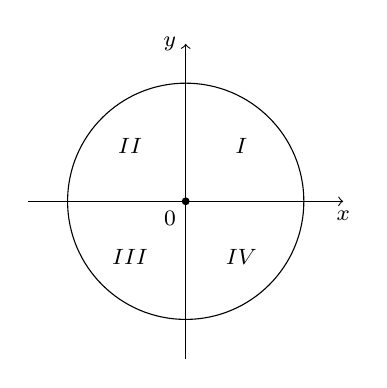
\begin{tikzpicture}[font=\footnotesize]
     \draw[->] (180:2)--(0:2) node[below] {$x$};
    \draw[->] (-90:2)--(90:2) node[left]  {$y$};
    \draw (0:0) circle  (1.5);
    \fill  (0:0) circle (0.05) node[below left] {$0$};
     \node at (45:1) {$I$};
    \node  at (135:1) {$II$};
    \node at  (225:1) {$III$};
    \node at  (-45:1) {$IV$};
   \end{tikzpicture}
  } 
 \loigiai{ 
  \begin{itemchoice}
   \itemch \immini{Điểm  biểu diễn của góc lượng giác có số đo $125 ^{\circ}$ là điểm $M$ thuộc góc phần tư thứ thứ II của đường tròn lượng giác thoả mãn $\widehat{AOM}=125 ^{\circ}$ .}
    {
   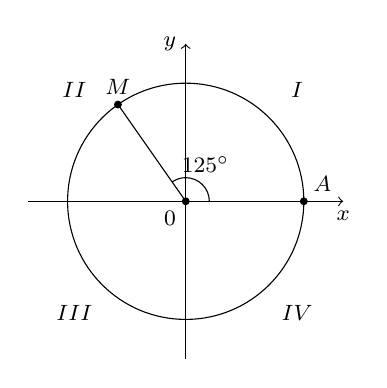
\begin{tikzpicture}[font=\footnotesize]
     \draw[->] (180:2)--(0:2) node[below]  {$x$};
     \draw[->] (-90:2)--(90:2) node[left]  {$y$};
     \draw  (0:0) circle (1.5);
     \fill (0:0) circle  (0.05) node[below left] {$0$};
     \node at (45:2)  {$I$};
     \node at (135:2) {$II$}; 
     \node at (225:2) {$III$}; 
     \node at (-45:2) {$IV$}; 
     \fill (125:1.5) circle (0.05) node[above]  {$M$};
     \fill (0:1.5) circle (0.05)  node[above right] {$A$};
      \draw (0:0)--(125:1.5)
      (0:0.3)  arc (0:125:0.3) node[above right] {$125^\circ$};
    \end{tikzpicture}
   } 
   \itemch \immini{ Ta có  $405 ^{\circ}=45 ^{\circ}+360 ^{\circ}$.
    Vì vậy điểm biểu diễn của góc lượng giác $405 ^{\circ}$ là điểm $N$ thuộc góc phần tư thứ $I$ của đường tròn lượng giác và thoả mãn $\widehat{AON}=45 ^{\circ}$ .}
   { 
   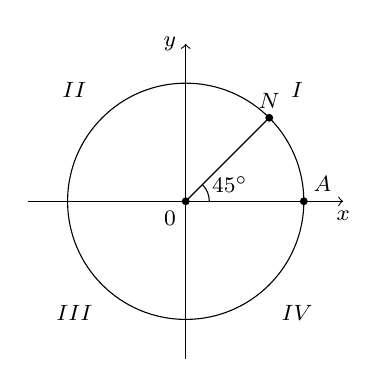
\begin{tikzpicture}[font=\footnotesize]
      \draw[->] (180:2)--(0:2) node[below] {$x$};
     \draw[->]  (-90:2)--(90:2) node[left] {$y$};
      \draw (0:0) circle (1.5);
     \fill (0:0) circle (0.05) node[below left] {$0$}; 
     \node  at (45:2) {$I$};
      \node at (135:2) {$II$};
      \node at (225:2) {$III$};
     \node at (-45:2) {$IV$}; 
     \fill (45:1.5) circle (0.05) node[above]  {$N$};
     \fill (0:1.5)  circle (0.05) node[above right] {$A$};
     \draw  (0:0)--(45:1.5)
      (0:0.3) arc (0:45:0.3) node[right] {$45^\circ$}; 
    \end{tikzpicture}
   } 
   \itemch \immini{Ta có  $\dfrac{19\pi}{3}=\dfrac{18\pi+\pi}{3}=\dfrac{\pi}{3}+3\cdot2\pi$.
   Vì vậy điểm biểu diễn của góc lượng giác $\dfrac{19\pi}{3}$ là điểm $P$ thuộc góc phần tư thứ $I$ của đường tròn  lượng giác và thoả mãn $\widehat{AOP}=\dfrac{\pi}{3}$ .}
    {
   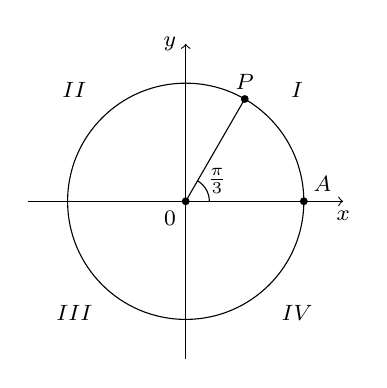
\begin{tikzpicture}[font=\footnotesize]
     \draw[->]  (180:2)--(0:2) node[below] {$x$};
     \draw[->]  (-90:2)--(90:2) node[left] {$y$};
     \draw  (0:0) circle (1.5);
     \fill (0:0) circle (0.05) node[below  left] {$0$};
     \node at (45:2) {$I$}; 
     \node at (135:2)  {$II$};
     \node at (225:2) {$III$}; 
     \node at  (-45:2) {$IV$};
     \fill (60:1.5) circle (0.05) node[above] {$P$}; 
     \fill (0:1.5)  circle (0.05) node[above right] {$A$};
      \draw (0:0)--(60:1.5)
      (0:0.3)  arc (0:60:0.3) node[right] {$\frac{\pi}{3}$};
    \end{tikzpicture}
    }
    \itemch \immini{
   Ta  có $-\dfrac{13\pi}{6}=\dfrac{-12\pi-\pi}{6}=-\dfrac{\pi}{6}-2\pi$.
   Vì vậy điểm biểu diễn của góc lượng giác $-\dfrac{13\pi}{6}$ là điểm $Q$ thuộc góc phần tư  thứ IV của đường tròn lượng giác và thoả mãn $\widehat{AOQ}=\dfrac{\pi}{6}$.}
    {
   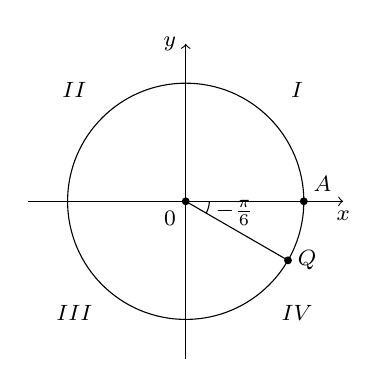
\begin{tikzpicture}[font=\footnotesize]
     \draw[->] (180:2)--(0:2) node[below] {$x$}; 
     \draw[->]  (-90:2)--(90:2) node[left] {$y$};
      \draw (0:0) circle (1.5);
     \fill (0:0) circle (0.05)  node[below left] {$0$};
     \node at  (45:2) {$I$};
     \node  at (135:2) {$II$};
     \node  at (225:2) {$III$};
     \node at  (-45:2) {$IV$};
      \fill (-30:1.5) circle (0.05) node[right] {$Q$};
     \fill (0:1.5) circle (0.05) node[above right] {$A$}; 
     \draw (0:0)--(-30:1.5) 
      (0:0.3) arc (0:-30:0.3) node[right] {$-\frac{\pi}{6}$}; 
    \end{tikzpicture}
   } 
  \end{itemchoice}
  }
\end{ex}

% nguồn: Ok_dungsai_lop11_Lan1
\begin{ex}%[1D1H1-4]%[ma:ba0f43cf]
 Cho đường tròn có bán kính $R=10\,\mathrm{cm}$.  Hãy cho biết tính đúng sai của mỗi khẳng định sau.
  \choiceTF
  {Chu vi của đường tròn bằng  $10\pi\,\mathrm{cm}$}
  {\True Cung trên đường tròn có  số đo $\dfrac{\pi}{2}$ có độ dài bằng $5\pi\,\mathrm{cm}$}
  {\True Cung có số đo $\dfrac{\pi}{6}$ có độ  dài bằng $\ell =\dfrac{5\pi}{3}\,\mathrm{cm}$ }
  {Cung có độ dài $\ell =4\pi\,\mathrm{cm}$  có số đo bằng $\dfrac{\pi}{5}$}
 \loigiai{ 
  \begin{itemchoice}
   \itemch Chu vi của đường tròn  là $C=2\pi\cdot R=20\pi\,\mathrm{cm}$.
   \itemch Cung có số đo  $\dfrac{\pi}{2}$ có độ dài $\ell =R\cdot \alpha =10\cdot \dfrac{\pi}{2}=5\pi\,\mathrm{cm}$.
   \itemch Cung có số đo  $\dfrac{\pi}{6}$ có độ dài bằng $\ell=10\cdot \dfrac{\pi}{6}=\dfrac{5\pi}{3}\,\mathrm{cm}$.
   \itemch Cung có  độ dài $\ell =4\pi\,\mathrm{cm}$ có số đo $\alpha=\dfrac{l}{R}=\dfrac{2\pi}{5}$.
  \end{itemchoice}
  }
\end{ex}

% nguồn: Ok_dungsai_lop11_Lan1
\begin{ex}%[1D1H1-4]%[ma:84cd567a]
 Các mệnh đề sau đây  \textbf{ĐÚNG} hay \textbf{SAI}?
 \choiceTF 
  {\True Điểm biểu diễn của góc lượng giác có số đo $218 ^{\circ}$ là điểm $M$ thuộc góc phần tư thứ III của đường tròn lượng giác  thoả mãn $\widehat{AOM}=218 ^{\circ}$}
  {Điểm biểu diễn của góc lượng giác có số đo $-405  ^{\circ}$ là điểm $N$ thuộc góc phần tư thứ IV của đường tròn lượng giác thoả mãn $\widehat{AON}=-45 ^{\circ}$}
  {\True Điểm biểu diễn của góc lượng giác có số đo $\dfrac{25\pi}{4}$ là điểm $P$ thuộc góc phần tư thứ I của đường  tròn lượng giác thoả mãn $\widehat{AOP}=\dfrac{\pi}{4}$}
  {Điểm biểu diễn của góc lượng giác có số đo $\dfrac{15\pi}{2}$ là điểm $Q(0;-1)$ thuộc đường tròn lượng  giác thoả mãn $\widehat{AOQ}=-\dfrac{\pi}{2}$}
 \loigiai{ 
  \begin{itemchoice}
   \itemch \immini{Điểm biểu diễn của góc lượng giác có số đo $218 ^{\circ}$ là điểm $M$ thuộc góc phần tư thứ III của đường tròn  lượng giác thoả mãn $\widehat{AOM}=218 ^{\circ}$. }{
   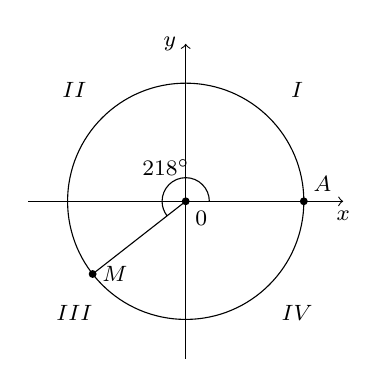
\begin{tikzpicture}[font=\footnotesize]
     \draw[->] (180:2)--(0:2)  node[below] {$x$};
      \draw[->] (-90:2)--(90:2) node[left] {$y$};
     \draw (0:0) circle  (1.5);
     \fill (0:0) circle (0.05) node[below  right] {$0$};
      \node at (45:2) {$I$};
     \node at  (135:2) {$II$};
     \node  at (225:2) {$III$};
     \node at (-45:2)  {$IV$};
     \fill (218:1.5) circle (0.05)  node[right] {$M$};
     \fill (0:1.5) circle  (0.05) node[above right] {$A$};
      \draw (0:0)--(218:1.5)
       (0:0.3) arc (0:218:0.3);
     \node[] at (120:0.5)  {$218^\circ$};
    \end{tikzpicture}
    }
   \itemch \immini{ Ta có $-405  ^{\circ}=-45 ^{\circ}-360 ^{\circ}$.
   Điểm biểu diễn của góc lượng giác có số đo $-405 ^{\circ}$ là điểm $N$ thuộc góc phần  tư thứ IV của đường tròn lượng giác thoả mãn $\widehat{AON}=45 ^{\circ}$. }{
   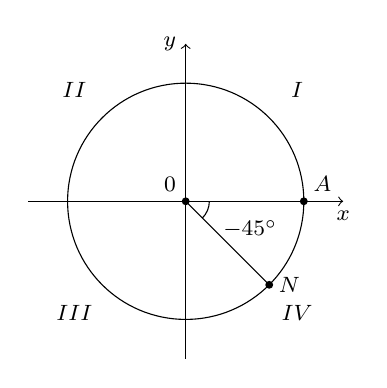
\begin{tikzpicture}[font=\footnotesize]
     \draw[->] (180:2)--(0:2)  node[below] {$x$};
     \draw[->] (-90:2)--(90:2) node[left]  {$y$};
     \draw (0:0)  circle (1.5);
     \fill  (0:0) circle (0.05) node[above left] {$0$};
     \node at  (45:2) {$I$};
      \node at (135:2) {$II$};
      \node at (225:2) {$III$};
     \node at (-45:2) {$IV$}; 
     \fill (-45:1.5) circle (0.05)  node[right] {$N$};
     \fill (0:1.5) circle  (0.05) node[above right] {$A$};
      \draw (0:0)--(-45:1.5)
      (0:0.3) arc (0:-45:0.3); 
     \node[right] at  (-45:0.5) {$-45^\circ$};
    \end{tikzpicture}
    }
   \itemch \immini{ Ta  có $\dfrac{25\pi}{4}=\dfrac{\pi+24\pi}{4}=\dfrac{\pi}{4}+6\pi$.
   Điểm  biểu diễn của góc lượng giác có số đo $\dfrac{25\pi}{4}$ là điểm $P$ thuộc góc phần tư thứ I của đường tròn lượng giác thoả mãn $\widehat{AOP}=\dfrac{\pi}{4}$. }{
   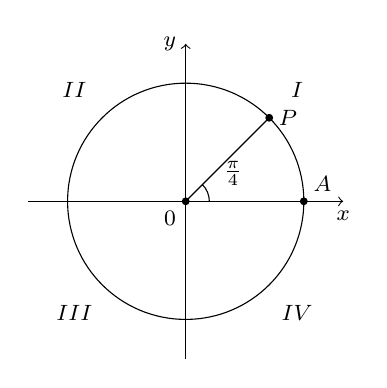
\begin{tikzpicture}[font=\footnotesize]
     \draw[->]  (180:2)--(0:2) node[below] {$x$};
      \draw[->] (-90:2)--(90:2) node[left] {$y$};
      \draw (0:0) circle (1.5);
     \fill (0:0)  circle (0.05) node[below left] {$0$};
     \node at (45:2)  {$I$};
     \node at (135:2) {$II$}; 
      \node at (225:2) {$III$};
     \node  at (-45:2) {$IV$};
     \fill (45:1.5) circle (0.05) node[right]  {$P$};
     \fill (0:1.5) circle (0.05)  node[above right] {$A$};
     \draw  (0:0)--(45:1.5)
      (0:0.3) arc (0:45:0.3); 
      \node[right] at (45:0.5) {$\frac{\pi}{4}$};
    \end{tikzpicture}
   } 
   \itemch \immini{Ta  có $\dfrac{15\pi}{2}=\dfrac{16\pi-\pi}{2}=-\dfrac{\pi}{2}+8\pi$.
   Điểm biểu diễn của góc lượng giác có  số đo $\dfrac{15\pi}{2}$ là điểm $Q(0;-1)$ thuộc đường tròn lượng giác thoả mãn $\widehat{AOQ}=\dfrac{\pi}{2}$. }{
   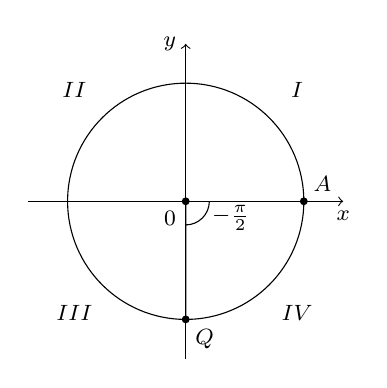
\begin{tikzpicture}[font=\footnotesize]
     \draw[->] (180:2)--(0:2) node[below]  {$x$};
     \draw[->]  (-90:2)--(90:2) node[left] {$y$};
     \draw (0:0)  circle (1.5);
     \fill  (0:0) circle (0.05) node[below left] {$0$};
      \node at (45:2) {$I$};
     \node at (135:2) {$II$}; 
     \node at (225:2) {$III$}; 
     \node at (-45:2) {$IV$}; 
     \fill (-90:1.5) circle (0.05)  node[below right] {$Q$};
     \fill (0:1.5) circle (0.05) node[above right] {$A$}; 
     \draw (0:0)--(-90:1.5) 
      (0:0.3)  arc (0:-90:0.3);
     \node[right]  at (-45:0.3) {$-\frac{\pi}{2}$};
    \end{tikzpicture}
    }
  \end{itemchoice}
  }
\end{ex}

% nguồn: Ok_dungsai_lop11_Lan1
\begin{ex}%[1D1H1-4]%[ma:11277127]
 Cho đường tròn có bán kính $R=10\,\mathrm{cm}$. Hãy cho biết tính  đúng sai của mỗi khẳng~định~sau.
 \choiceTF 
  {\True Cung trên đường tròn  có số đo $\dfrac{\pi}{2}$ có độ dài bằng $5\pi\,\mathrm{cm}$}
   {Chu vi của đường tròn bằng $10\pi\,\mathrm{cm}$}
  {\True Cung có số đo $\dfrac{\pi}{6}$ có  độ dài bằng $\ell =\dfrac{5\pi}{3}\,\mathrm{cm}$ }
  {Cung có độ dài  $\ell =4\pi\,\mathrm{cm}$ có số đo bằng $\dfrac{\pi}{5}$}
 \loigiai{ 
  \begin{itemchoice}
   \itemch Cung có số đo $\dfrac{\pi}{2}$ có  độ dài $\ell =R\cdot \alpha =10\cdot \dfrac{\pi}{2}=5\pi\,\mathrm{cm}$.
    \itemch Chu vi của đường tròn là $C=2\pi\cdot R=20\pi\,\mathrm{cm}$.
   \itemch Cung có số đo $\dfrac{\pi}{6}$ có độ  dài bằng $\ell=10\cdot \dfrac{\pi}{6}=\dfrac{5\pi}{3}\,\mathrm{cm}$.
   \itemch Cung có độ dài $\ell  =4\pi\,\mathrm{cm}$ có số đo $\alpha=\dfrac{l}{R}=\dfrac{2\pi}{5}$.
  \end{itemchoice}
  }
\end{ex}

% nguồn: Ok_dungsai_lop11_Lan2
\begin{ex}%[1D1H1-4]%[ma:537a627c]
	Xét tính đúng sai của các mệnh  đề sau:
	 \choiceTF
		{\True Trên đường tròn bán kính bằng $4$, cung có số đo $\dfrac{\pi}{8}$ thì có độ dài là  $\dfrac{\pi}{2}$}
		 {\True Trên đường tròn bán kính bằng $4$, cung có số đo $45^\circ$ thì có độ dài là $\pi $}
		{Trên  đường tròn bán kính bằng $4$, cung có số đo $\dfrac{\pi}{10}$ thì có độ dài là $\dfrac{\pi}{2}$}
		{\True Trên đường tròn bán  kính bằng $10$, cung có số đo $\dfrac{\pi}{5}$ thì có độ dài là $2\pi $}
	\loigiai{ 
		Cung có số đo $\alpha $ rad của đường tròn bán kính $R$  có độ dài $ l=R\cdot\alpha $.
		\begin{itemchoice}
			 \itemch \textbf{Đúng.}\\
			 Ta có $\alpha =\dfrac{\pi}{8}$; $R=4$ thì $ l=R\cdot\alpha =\dfrac{\pi}{2}$.
			\itemch \textbf{Đúng.}\\ 
			Ta có  $45^\circ=\dfrac{\pi}{4}$ rad; $ l=R\cdot\alpha =\pi $.
			 \itemch \textbf{Sai.}\\
			Ta có  $ l=R\cdot\alpha =\dfrac{2\pi}{5}$.
			\itemch \textbf{Đúng.}\\ 
			Ta có $ l=R\cdot\alpha  =2\pi $.
		\end{itemchoice}
	 }
\end{ex}


%%%%%%%%%%%%%%%% TRẢ LỜI NGẮN %%%%%%%%%%%%%%%%

% nguồn: Ok_TraLoiNgan_Lop11_Lan2
\begin{ex}%[1D1H1-4]%[ma:d11fbc74]
	Huyện lị Quản Bạ tỉnh Hà Giang và huyện lị Cái Nước tỉnh Cà Mau  cùng nằm ở $105^{\circ}$ kinh đông, nhưng Quản Bạ ở $23^{\circ}$ vĩ bắc, Cái Nước ở vĩ độ $9^{\circ}$ bắc. Hãy tính độ dài của cung kinh tuyến nối hai huyện lị đó (khoảng cách theo đường chim bay), coi Trái Đất có bán kính $6278$\,km. (Kết quả làm tròn đến hàng đơn vị)
	\shortans{1558} 
	\loigiai{ 
		Góc ở tâm chắn cung kinh tuyến nối huyện Quản Bạ tỉnh Hà Giang  và huyện Cái Nước tỉnh Cà Mau có số đo bằng $23^{\circ}-9^{\circ}=14^{\circ}$.\\
	Vậy độ  dài cung kinh tuyến đó bằng $\dfrac{6378\cdot 14\cdot \pi}{180} \approx 1558$\,km.}
\end{ex}

% nguồn: Ok_TraLoiNgan_Lop11_Lan1
\begin{ex}%[1D1V1-4]%[ma:e51f3e37]
	\immini{ Một cái đồng hồ treo tường có đường kính bằng $60$ cm, ta xem vành ngoài chiếc đồng  hồ là một đường tròn với các điểm $A$, $B$, $C$ lần lượt tương ứng với vị trí các số $2$, $9$, $4$.
	Tính độ dài các cung nhỏ $AB$ (kết quả tính theo đơn vị centimét và làm tròn đến hàng phần trăm).}{\begin{tikzpicture}[r/.style={font=\sffamily,
			inner  sep=0,
			rotate=-30*\x, 
			 anchor=north},
			declare  function = {hour= 10; minute= 15; second =45;},
			 s/.style={even odd rule,
			top  color= black,
			bottom color= black, 
			middle  color=white},scale=0.8]
		 \pgfmathsetmacro{\hourhand}{hour}
		 \pgfmathsetmacro{\minutehand}{minute}
		\pgfmathsetmacro{\secondhand}{second} 
		\shade[s,shading  angle=-10] circle (21mm) circle (22mm);
		\shade[s,shading angle=15] circle (22mm)  circle (25mm);
		\foreach\x[evaluate={\xf=int (5*\x);}]  in{1,...,12}{
			 \draw ({30*(3-\x)}:19mm) node[r,anchor=south,scale=0.5,inner sep=1pt] {\xf}
			 node[r,scale=1.5,xscale=0.85] at ({30*(3-\x)}:1.8cm)
			{\uppercase\expandafter{\romannumeral\x}}; 
			\ifodd\x\else\draw (30*\x:18mm-2.5ex)--++(30*\x:-1mm);  \fi
		} 
		\foreach\x  in{1,...,60}{\draw (6*\x:18mm)--++(6*\x:1mm);}
		\draw circle (18mm) circle (19mm) circle (18mm-2.5ex)  circle (17mm-2.5ex);
		\begin{scope}[rotate around={-6*(\minutehand):(0,0)}]
			 \fill (0.5mm,0) to[out=90,in=-100] (80:1.2cm) to[in=-80,out=120] (90:1.75cm)
				to[out=-100,in=60]  (100:1.2cm) to[in=90,out=-80](-0.5mm,0);
		\end{scope}
		\begin{scope}[rotate around={-30*(\hourhand+\minutehand/60):(0,0)}]
			\fill (0.5mm,0) to[out=90,in=-150] (70:6mm) to[in=-80,out=120]  (90:1.4cm)
				 to[out=-100,in=60] (110:6mm) to[in=90,out=-30](-0.5mm,0);
		\end{scope}
		\draw[thick,-{Kite[scale=0.8]}] (0,0)  -- (90-6*\secondhand:1.8cm);
		\filldraw[fill=white]circle  (1mm);
		 \node at (32:30mm) {$A$};
		\node at  (180:30mm) {$B$};
		\node at  (-32:30mm) {$C$};
	\end{tikzpicture}
	} 
	 \shortans{78,5}
	\loigiai{ 
		Bán kính đường tròn là $R=\dfrac{60}{2}=30  $ (cm).\\[2pt]
		Ta có $\widehat{AOB}=150 ^{\circ}=\dfrac{150\pi}{180}$ rad $=\dfrac{5\pi}{6}  $ rad.\\
		Suy ra độ dài cung nhỏ $AB$ là $l_{\wideparen{AB}}=R\cdot  \widehat{AOB}=30\cdot \dfrac{5\pi}{6}=25\pi \approx 78{,}54 $ (cm).
	 }
\end{ex}


%%%%%%%%%%%%%%%% TỰ LUẬN %%%%%%%%%%%%%%%%

% nguồn: Ok_TuanLuan_Toan11_Lan2
\begin{ex}%[1D1N1-4]%[ma:6507aa39]
	Một đu quay ở công viên có bán kính bằng $10$ m. Tốc độ  của đu quay là $3$ vòng/phút. Hỏi mất bao lâu để đu quay quay được góc $270^{\circ}$?
	\loigiai{ 
		Tính được $270^{\circ}=\dfrac{270}{180} \pi=\dfrac{3}{2} \pi=\dfrac{3}{4}.2\pi$.  \\
		Vậy đu quay quay  được góc $270^{\circ}$ khi nó quay được $\dfrac{3}{4}$ vòng.\\
		Đu quay quay được $1$  vòng trong $\dfrac{1}{3}$ phút.\\
		Đu  quay quay được $\dfrac{3}{4}$ vòng trong $\dfrac{3}{4} \cdot \dfrac{1}{3}=\dfrac{1}{4}$ phút.
	 }
\end{ex}

% nguồn: Ok_TuanLuan_Toan11_Lan2
\begin{ex}%[1D1N1-4]%[ma:caa35061]
	Một đường tròn có bán kính bằng $10$ cm. Tính độ dài của cung tròn có  số đo $30^{\circ}$. (làm tròn kết quả đến hàng phần trăm)
	\loigiai{ 
		Độ dài của cung tròn có số đo $30^{\circ}$ là $l=\dfrac{30\cdot \pi \cdot R}{180} = \dfrac{30\cdot \pi \cdot 10}{180} \approx 5{,}26$  cm.
	 }
\end{ex}

% nguồn: Ok_TuanLuan_Toan11_Lan2
\begin{ex}%[1D1N1-4]%[ma:ba5ba364]
	 Một bánh xe máy có đường kính $60$. Nếu xe chạy với vận tốc $50\,(\mathrm{km}/h)$ thì trong $5$ giây bánh xe quay được bao nhiêu vòng.
	 \loigiai{
		Trong một phút bánh xe quay được $\left[\dfrac{50\cdot 1\,000}{3\,600}:(0{,}6\cdot \pi)\right]\cdot 5\approx 36{,}9$. 
	} 
\end{ex}

% nguồn: Ok_TuanLuan_Toan11_Lan2
\begin{ex}%[1D1N1-4]%[ma:2594645f]
	Trả lời các câu hỏi được nêu ra trong các trường  hợp sau:
	\begin{enumerate}
		\item Trên đường tròn bán kính  $r=5$. Tìm độ dài của cung đo $\dfrac{\pi}{8}$.
		\item Trên đường tròn bán kính $r=15$.  Tìm độ dài của cung có số đo $50^{\circ}$.
		\item Một cung tròn có độ dài bằng $2$ lần bán kính. Tìm số đo  rađian của cung tròn đó.
		 \item Một đường tròn có $r=30$. Tìm độ dài của một cung trên đường tròn có số đo $1{,}5\,\mathrm{rad}$.
		\item Một đường  tròn có bán kính $R=\dfrac{10}{\pi}\, \mathrm{cm}$. Tìm độ dài của cung $\dfrac{\pi}{2}$ trên đường tròn.
		\item Một đường tròn có bán kính $R=10\,\mathrm{cm}$. Tìm độ dài cung $40^{\circ}$ trên đường tròn  đó.
	\end{enumerate}
	 \loigiai{
		\begin{enumerate}
			\item Độ dài cung $AB$ có  số đo cung $AB$ bằng $n$ độ: $l=r \cdot n=5\cdot \dfrac{\pi}{8}$.
			\item $l=\dfrac{\pi \cdot r \cdot n^{\circ}}{180^{\circ}}=\dfrac{\pi 15\cdot 50}{180}=\dfrac{25\pi}{6}$. 
			\item Ta có, cung tròn có độ dài bằng bán kính thì  có số đo $1$ radian. \\
			Vậy cung tròn đó có số đo là $2$ radian. 
			\item Áp  dụng công thức $\ell=\alpha R$ nên ta được độ dài cung tròn là $45$ cm.
			 \item Độ dài cung có số đo $\alpha$ là $\ell=\alpha \cdot R\Rightarrow \ell=\dfrac{\pi}{2} \cdot \dfrac{10}{\pi}=5\,(\mathrm{cm})$.
			\item Đổi đơn vị $40^{\circ} \Rightarrow \dfrac{40\cdot \pi}{180}=\dfrac{2\pi}{9} \Rightarrow$  độ dài cung $\ell=\dfrac{2\pi}{9} \cdot 10=\dfrac{20\pi}{9}=6{,}9813\,(\mathrm{cm})$.
		\end{enumerate}
	} 
\end{ex}

% nguồn: Ok_TuanLuan_Toan11_Lan2
\begin{ex}%[1D1H1-4]%[ma:83812339]
	Một đồng hồ treo tường  có kim giờ dài $10{,}25\,\mathrm{cm}$, kim phút dài $13{,}25\,\mathrm{cm}$. Trong $30$ phút kim giờ vạch nên cung tròn có độ dài bao nhiêu?
	\begin{center}
		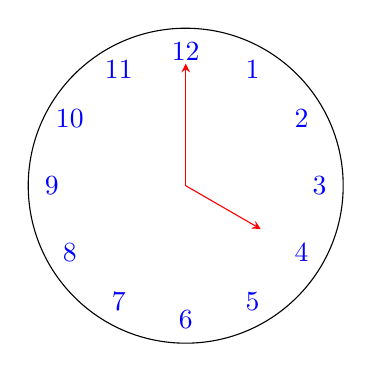
\begin{tikzpicture}[>=stealth]
				 \draw (0,0) circle (2cm);
				\draw[->,red] (0,0) --  ({1.55*cos (90)},{1.55*sin (90)});
				\draw[->,red] (0,0) -- ({1.1*cos (-30)},{1.1*sin (-30)}); 
				 \draw[blue]({1.7*cos (-30)},{1.7*sin (-30)}) node{$4$};
				\draw[blue]({1.7*cos  (0)},{1.7*sin (0)}) node{$3$};
				\draw[blue]({1.7*cos (30)},{1.7*sin (30)}) node{$2$}; 
				\draw[blue]({1.7*cos (60)},{1.7*sin  (60)}) node{$1$};
				\draw[blue]({1.7*cos (90)},{1.7*sin (90)})  node{$12$};
				\draw[blue]({1.7*cos  (120)},{1.7*sin (120)}) node{$11$};
				\draw[blue]({1.7*cos (150)},{1.7*sin (150)})  node{$10$};
				\draw[blue]({1.7*cos (180)},{1.7*sin (180)}) node{$9$}; 
				 \draw[blue]({1.7*cos (210)},{1.7*sin (210)}) node{$8$};
				\draw[blue]({1.7*cos (240)},{1.7*sin (240)}) node{$7$}; 
				\draw[blue]({1.7*cos  (270)},{1.7*sin (270)}) node{$6$};
				 \draw[blue]({1.7*cos (300)},{1.7*sin (300)}) node{$5$};
			\end{tikzpicture}
	\end{center}
	 \loigiai{
		Trong $6$ giờ kim giờ  vạch nên một cung có số đo là $\pi\,(\mathrm{rad})$, vậy trong $30$ phút kim giờ vạch nên cung có số đo là $\dfrac{\pi}{12}\,(\mathrm{rad})$. Khi đó độ dài cung tròn mà kim giờ vạch ra trong $30$ phút là
		$$ 
		\ell=R \cdot \alpha \Rightarrow \ell=10{,}25 \cdot  \dfrac{\pi}{12}=2{,}68\,(\mathrm{cm}).
		$$ 
	 }
\end{ex}
